\chapter{Giới thiệu}
\label{ch:gioi-thieu}
% Đề mục 4: Bối cảnh; game, luật và ý nghĩa; mục tiêu, câu hỏi nghiên cứu; phạm vi; sản phẩm.
% Hình và các con số ở mục Đặc điểm trò chơi: uv run python report/scripts/ve_hinh_gioi_thieu.py
% TRƯỚC KHI NỘP: cập nhật cột trạng thái ở Bảng tab:gt-cap, tab:gt-san-pham và ngày ghi trong chú thích.

\section{Bối cảnh}
\label{sec:gt-boi-canh}
Trò chơi hai người có thông tin đầy đủ là môi trường thử nghiệm lâu đời của trí tuệ nhân tạo \cite{russell2021aima}. Luật chơi được định nghĩa chính xác nên máy tính mô phỏng được với chi phí thấp, kết quả của mỗi ván là thắng, hoà hoặc thua nên sức mạnh đo được trực tiếp bằng đối đầu, và tác tử có thể tự sinh dữ liệu mà không phụ thuộc vào nguồn bên ngoài. Nhờ vậy, nhiều phương pháp rất khác nhau có thể được so sánh trên cùng một bài toán.

Trên môi trường này đã hình thành ba hướng tiếp cận chính. Hướng thứ nhất là \textbf{tìm kiếm có tri thức do con người viết}: Minimax kết hợp cắt tỉa Alpha-Beta \cite{knuth1975alphabeta} duyệt cây đến một độ sâu giới hạn rồi dùng hàm lượng giá để chấm thế cờ ở lá. Hướng thứ hai là \textbf{tìm kiếm dựa trên lấy mẫu}: tìm kiếm cây Monte Carlo, tiêu biểu là UCT \cite{kocsis2006uct,browne2012mcts}, ước lượng giá trị nước đi từ kết quả các ván mô phỏng thay vì từ hàm lượng giá viết tay. Hướng thứ ba là \textbf{học từ dữ liệu}: mạng nơ-ron học chính sách và giá trị từ ván của chuyên gia hoặc từ tự chơi. AlphaGo \cite{silver2016alphago} kết hợp mạng nơ-ron với tìm kiếm cây Monte Carlo; AlphaGo Zero và AlphaZero \cite{silver2017alphagozero,silver2018alphazero} tiếp tục bỏ dữ liệu của con người, chỉ học bằng self-play từ luật chơi.

Các kết quả trên đạt được với ngân sách tính toán mà một đồ án môn học không thể lặp lại, nhưng câu hỏi đặt ra ở quy mô nhỏ vẫn có giá trị: với cùng một trò chơi và cùng một ngân sách, tri thức viết tay, lấy mẫu và mô hình tự học khác nhau bao nhiêu về chất lượng nước đi và chi phí tính toán, và phần nào của mỗi phương pháp thực sự tạo ra khác biệt. Trả lời được câu hỏi này đòi hỏi các tác tử phải chạy trên cùng một engine, qua cùng một giao diện lập trình và được chấm bằng cùng một giải đấu.

Đề tài ``Xây dựng và đánh giá Game AI đa cấp độ'' của học phần Trí tuệ nhân tạo nâng cao đặt ra đúng yêu cầu đó, với tám cấp tác tử từ Random đến AlphaZero-inspired. Đề bài nêu rõ các cấp thể hiện mức độ phức tạp của phương pháp, không mặc nhiên tương ứng với sức mạnh thực tế. Vì vậy báo cáo này coi thứ hạng giữa các cấp là điều cần đo, không phải điều đã biết trước.

\section{Trò chơi Caro 11×11}
\label{sec:gt-tro-choi}
Trong các trò chơi đề bài gợi ý, nhóm chọn Caro (Gomoku) với mức độ khó khá--cao. Đề bài khuyến nghị bàn 9×9 hoặc 11×11 và yêu cầu quy định chính xác điều kiện thắng cùng luật chặn; nhóm chọn bàn 11×11 và không áp dụng luật chặn hai đầu, gọi là \emph{luật tự do}.

\subsection{Luật chơi}
\label{sec:gt-luat}
Luật áp dụng trong toàn bộ đề tài gồm các điểm sau:
\begin{itemize}
  \item \textbf{Bàn cờ:} lưới 11×11, tổng cộng 121 ô, ban đầu trống. Trong báo cáo, cột được ghi từ A đến K, hàng từ 1 đến 11; riêng phần mã nguồn dùng toạ độ $(r, c)$ đánh số từ 0, ví dụ ô D4 là $(3, 3)$.
  \item \textbf{Lượt đi:} X đi trước, O đi sau, luân phiên mỗi lượt đặt một quân vào một ô trống bất kỳ. Quân đã đặt không di chuyển và không bị bắt. Bên đến lượt không được bỏ lượt.
  \item \textbf{Thắng:} bên đầu tiên có từ 5 quân liên tiếp trở lên theo hàng ngang, cột dọc hoặc một trong hai đường chéo thì thắng, và ván kết thúc ngay. Dãy dài hơn 5 quân vẫn thắng, dãy bị quân đối thủ chặn cả hai đầu cũng vẫn thắng.
  \item \textbf{Hoà:} bàn đầy sau 121 nước (X 61 quân, O 60 quân) mà chưa bên nào thắng.
  \item \textbf{Nước bất hợp lệ:} đặt vào ô đã có quân, đặt ngoài bàn hoặc đi sau khi ván đã kết thúc đều bị engine từ chối.
\end{itemize}

Ván ngắn nhất có thể kết thúc ở nước thứ 9, khi X đặt quân thứ năm. Hình~\ref{fig:gt-ban}a là một ván X thắng bằng dãy chéo D4--H8 dù O đã chặn cả hai đầu ở C3 và I9. Trong các biến thể phổ biến ở Việt Nam, thế này có thể không được công nhận là thắng; Bảng~\ref{tab:gt-bien-the} so sánh các biến thể đó với luật của đề tài.

\begin{figure}[!htb]
  \centering
  \begin{subfigure}[t]{.49\textwidth}
    \centering
    % Sinh bởi report/scripts/ve_hinh_gioi_thieu.py, không sửa tay.
\definecolor{gtX}{HTML}{1E293B}
\definecolor{gtO}{HTML}{C81E1E}
\definecolor{gtThang}{HTML}{1B7F4B}
\definecolor{gtVang}{HTML}{FDE68A}
\definecolor{gtNhiet}{HTML}{4A90C8}
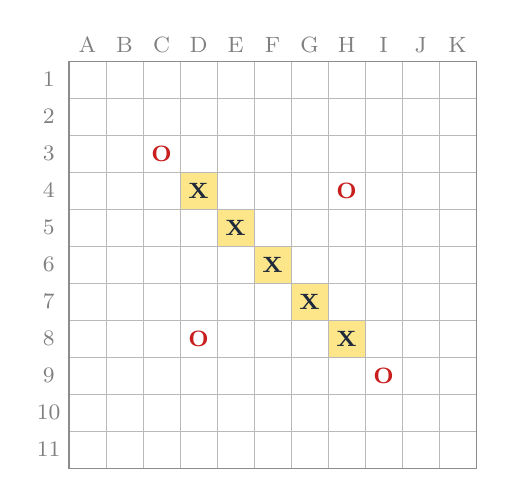
\begin{tikzpicture}[x=.47cm, y=.47cm]
\fill[gtVang] (5,-5) rectangle ++(1,-1);
\fill[gtVang] (4,-4) rectangle ++(1,-1);
\fill[gtVang] (6,-6) rectangle ++(1,-1);
\fill[gtVang] (3,-3) rectangle ++(1,-1);
\fill[gtVang] (7,-7) rectangle ++(1,-1);
\draw[gray!55, line width=.3pt, step=1] (0,0) grid (11,-11); \draw[gray!90] (0,0) rectangle (11,-11);
\node[font=\footnotesize, text=gray] at (0.5,.45) {A};
\node[font=\footnotesize, text=gray] at (1.5,.45) {B};
\node[font=\footnotesize, text=gray] at (2.5,.45) {C};
\node[font=\footnotesize, text=gray] at (3.5,.45) {D};
\node[font=\footnotesize, text=gray] at (4.5,.45) {E};
\node[font=\footnotesize, text=gray] at (5.5,.45) {F};
\node[font=\footnotesize, text=gray] at (6.5,.45) {G};
\node[font=\footnotesize, text=gray] at (7.5,.45) {H};
\node[font=\footnotesize, text=gray] at (8.5,.45) {I};
\node[font=\footnotesize, text=gray] at (9.5,.45) {J};
\node[font=\footnotesize, text=gray] at (10.5,.45) {K};
\node[font=\footnotesize, text=gray] at (-.55,-0.5) {1};
\node[font=\footnotesize, text=gray] at (-.55,-1.5) {2};
\node[font=\footnotesize, text=gray] at (-.55,-2.5) {3};
\node[font=\footnotesize, text=gray] at (-.55,-3.5) {4};
\node[font=\footnotesize, text=gray] at (-.55,-4.5) {5};
\node[font=\footnotesize, text=gray] at (-.55,-5.5) {6};
\node[font=\footnotesize, text=gray] at (-.55,-6.5) {7};
\node[font=\footnotesize, text=gray] at (-.55,-7.5) {8};
\node[font=\footnotesize, text=gray] at (-.55,-8.5) {9};
\node[font=\footnotesize, text=gray] at (-.55,-9.5) {10};
\node[font=\footnotesize, text=gray] at (-.55,-10.5) {11};
\node[text=gtX, font=\bfseries\footnotesize] at (5.5,-5.5) {X};
\node[text=gtX, font=\bfseries\footnotesize] at (4.5,-4.5) {X};
\node[text=gtX, font=\bfseries\footnotesize] at (6.5,-6.5) {X};
\node[text=gtX, font=\bfseries\footnotesize] at (3.5,-3.5) {X};
\node[text=gtX, font=\bfseries\footnotesize] at (7.5,-7.5) {X};
\node[text=gtO, font=\bfseries\footnotesize] at (2.5,-2.5) {O};
\node[text=gtO, font=\bfseries\footnotesize] at (8.5,-8.5) {O};
\node[text=gtO, font=\bfseries\footnotesize] at (7.5,-3.5) {O};
\node[text=gtO, font=\bfseries\footnotesize] at (3.5,-7.5) {O};
\end{tikzpicture}

    \caption{Một ván kết thúc: X thắng bằng dãy chéo D4--H8.}
  \end{subfigure}\hfill
  \begin{subfigure}[t]{.49\textwidth}
    \centering
    % Sinh bởi report/scripts/ve_hinh_gioi_thieu.py, không sửa tay.
\definecolor{gtX}{HTML}{1E293B}
\definecolor{gtO}{HTML}{C81E1E}
\definecolor{gtThang}{HTML}{1B7F4B}
\definecolor{gtVang}{HTML}{FDE68A}
\definecolor{gtNhiet}{HTML}{4A90C8}
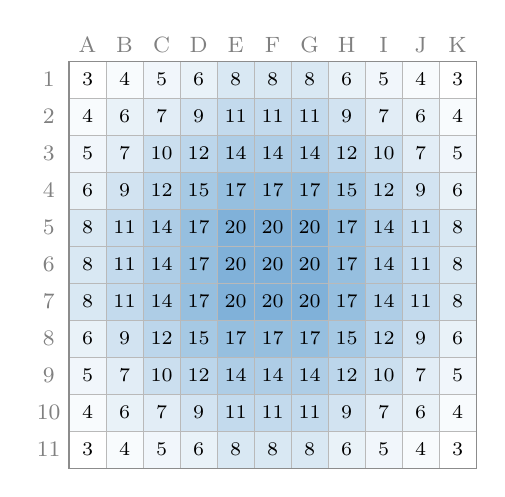
\begin{tikzpicture}[x=.47cm, y=.47cm]
\fill[gtNhiet!0] (0,0) rectangle ++(1,-1);
\node[font=\scriptsize] at (0.5,-0.5) {3};
\fill[gtNhiet!4] (1,0) rectangle ++(1,-1);
\node[font=\scriptsize] at (1.5,-0.5) {4};
\fill[gtNhiet!8] (2,0) rectangle ++(1,-1);
\node[font=\scriptsize] at (2.5,-0.5) {5};
\fill[gtNhiet!12] (3,0) rectangle ++(1,-1);
\node[font=\scriptsize] at (3.5,-0.5) {6};
\fill[gtNhiet!21] (4,0) rectangle ++(1,-1);
\node[font=\scriptsize] at (4.5,-0.5) {8};
\fill[gtNhiet!21] (5,0) rectangle ++(1,-1);
\node[font=\scriptsize] at (5.5,-0.5) {8};
\fill[gtNhiet!21] (6,0) rectangle ++(1,-1);
\node[font=\scriptsize] at (6.5,-0.5) {8};
\fill[gtNhiet!12] (7,0) rectangle ++(1,-1);
\node[font=\scriptsize] at (7.5,-0.5) {6};
\fill[gtNhiet!8] (8,0) rectangle ++(1,-1);
\node[font=\scriptsize] at (8.5,-0.5) {5};
\fill[gtNhiet!4] (9,0) rectangle ++(1,-1);
\node[font=\scriptsize] at (9.5,-0.5) {4};
\fill[gtNhiet!0] (10,0) rectangle ++(1,-1);
\node[font=\scriptsize] at (10.5,-0.5) {3};
\fill[gtNhiet!4] (0,-1) rectangle ++(1,-1);
\node[font=\scriptsize] at (0.5,-1.5) {4};
\fill[gtNhiet!12] (1,-1) rectangle ++(1,-1);
\node[font=\scriptsize] at (1.5,-1.5) {6};
\fill[gtNhiet!16] (2,-1) rectangle ++(1,-1);
\node[font=\scriptsize] at (2.5,-1.5) {7};
\fill[gtNhiet!25] (3,-1) rectangle ++(1,-1);
\node[font=\scriptsize] at (3.5,-1.5) {9};
\fill[gtNhiet!33] (4,-1) rectangle ++(1,-1);
\node[font=\scriptsize] at (4.5,-1.5) {11};
\fill[gtNhiet!33] (5,-1) rectangle ++(1,-1);
\node[font=\scriptsize] at (5.5,-1.5) {11};
\fill[gtNhiet!33] (6,-1) rectangle ++(1,-1);
\node[font=\scriptsize] at (6.5,-1.5) {11};
\fill[gtNhiet!25] (7,-1) rectangle ++(1,-1);
\node[font=\scriptsize] at (7.5,-1.5) {9};
\fill[gtNhiet!16] (8,-1) rectangle ++(1,-1);
\node[font=\scriptsize] at (8.5,-1.5) {7};
\fill[gtNhiet!12] (9,-1) rectangle ++(1,-1);
\node[font=\scriptsize] at (9.5,-1.5) {6};
\fill[gtNhiet!4] (10,-1) rectangle ++(1,-1);
\node[font=\scriptsize] at (10.5,-1.5) {4};
\fill[gtNhiet!8] (0,-2) rectangle ++(1,-1);
\node[font=\scriptsize] at (0.5,-2.5) {5};
\fill[gtNhiet!16] (1,-2) rectangle ++(1,-1);
\node[font=\scriptsize] at (1.5,-2.5) {7};
\fill[gtNhiet!29] (2,-2) rectangle ++(1,-1);
\node[font=\scriptsize] at (2.5,-2.5) {10};
\fill[gtNhiet!37] (3,-2) rectangle ++(1,-1);
\node[font=\scriptsize] at (3.5,-2.5) {12};
\fill[gtNhiet!45] (4,-2) rectangle ++(1,-1);
\node[font=\scriptsize] at (4.5,-2.5) {14};
\fill[gtNhiet!45] (5,-2) rectangle ++(1,-1);
\node[font=\scriptsize] at (5.5,-2.5) {14};
\fill[gtNhiet!45] (6,-2) rectangle ++(1,-1);
\node[font=\scriptsize] at (6.5,-2.5) {14};
\fill[gtNhiet!37] (7,-2) rectangle ++(1,-1);
\node[font=\scriptsize] at (7.5,-2.5) {12};
\fill[gtNhiet!29] (8,-2) rectangle ++(1,-1);
\node[font=\scriptsize] at (8.5,-2.5) {10};
\fill[gtNhiet!16] (9,-2) rectangle ++(1,-1);
\node[font=\scriptsize] at (9.5,-2.5) {7};
\fill[gtNhiet!8] (10,-2) rectangle ++(1,-1);
\node[font=\scriptsize] at (10.5,-2.5) {5};
\fill[gtNhiet!12] (0,-3) rectangle ++(1,-1);
\node[font=\scriptsize] at (0.5,-3.5) {6};
\fill[gtNhiet!25] (1,-3) rectangle ++(1,-1);
\node[font=\scriptsize] at (1.5,-3.5) {9};
\fill[gtNhiet!37] (2,-3) rectangle ++(1,-1);
\node[font=\scriptsize] at (2.5,-3.5) {12};
\fill[gtNhiet!49] (3,-3) rectangle ++(1,-1);
\node[font=\scriptsize] at (3.5,-3.5) {15};
\fill[gtNhiet!58] (4,-3) rectangle ++(1,-1);
\node[font=\scriptsize] at (4.5,-3.5) {17};
\fill[gtNhiet!58] (5,-3) rectangle ++(1,-1);
\node[font=\scriptsize] at (5.5,-3.5) {17};
\fill[gtNhiet!58] (6,-3) rectangle ++(1,-1);
\node[font=\scriptsize] at (6.5,-3.5) {17};
\fill[gtNhiet!49] (7,-3) rectangle ++(1,-1);
\node[font=\scriptsize] at (7.5,-3.5) {15};
\fill[gtNhiet!37] (8,-3) rectangle ++(1,-1);
\node[font=\scriptsize] at (8.5,-3.5) {12};
\fill[gtNhiet!25] (9,-3) rectangle ++(1,-1);
\node[font=\scriptsize] at (9.5,-3.5) {9};
\fill[gtNhiet!12] (10,-3) rectangle ++(1,-1);
\node[font=\scriptsize] at (10.5,-3.5) {6};
\fill[gtNhiet!21] (0,-4) rectangle ++(1,-1);
\node[font=\scriptsize] at (0.5,-4.5) {8};
\fill[gtNhiet!33] (1,-4) rectangle ++(1,-1);
\node[font=\scriptsize] at (1.5,-4.5) {11};
\fill[gtNhiet!45] (2,-4) rectangle ++(1,-1);
\node[font=\scriptsize] at (2.5,-4.5) {14};
\fill[gtNhiet!58] (3,-4) rectangle ++(1,-1);
\node[font=\scriptsize] at (3.5,-4.5) {17};
\fill[gtNhiet!70] (4,-4) rectangle ++(1,-1);
\node[font=\scriptsize] at (4.5,-4.5) {20};
\fill[gtNhiet!70] (5,-4) rectangle ++(1,-1);
\node[font=\scriptsize] at (5.5,-4.5) {20};
\fill[gtNhiet!70] (6,-4) rectangle ++(1,-1);
\node[font=\scriptsize] at (6.5,-4.5) {20};
\fill[gtNhiet!58] (7,-4) rectangle ++(1,-1);
\node[font=\scriptsize] at (7.5,-4.5) {17};
\fill[gtNhiet!45] (8,-4) rectangle ++(1,-1);
\node[font=\scriptsize] at (8.5,-4.5) {14};
\fill[gtNhiet!33] (9,-4) rectangle ++(1,-1);
\node[font=\scriptsize] at (9.5,-4.5) {11};
\fill[gtNhiet!21] (10,-4) rectangle ++(1,-1);
\node[font=\scriptsize] at (10.5,-4.5) {8};
\fill[gtNhiet!21] (0,-5) rectangle ++(1,-1);
\node[font=\scriptsize] at (0.5,-5.5) {8};
\fill[gtNhiet!33] (1,-5) rectangle ++(1,-1);
\node[font=\scriptsize] at (1.5,-5.5) {11};
\fill[gtNhiet!45] (2,-5) rectangle ++(1,-1);
\node[font=\scriptsize] at (2.5,-5.5) {14};
\fill[gtNhiet!58] (3,-5) rectangle ++(1,-1);
\node[font=\scriptsize] at (3.5,-5.5) {17};
\fill[gtNhiet!70] (4,-5) rectangle ++(1,-1);
\node[font=\scriptsize] at (4.5,-5.5) {20};
\fill[gtNhiet!70] (5,-5) rectangle ++(1,-1);
\node[font=\scriptsize] at (5.5,-5.5) {20};
\fill[gtNhiet!70] (6,-5) rectangle ++(1,-1);
\node[font=\scriptsize] at (6.5,-5.5) {20};
\fill[gtNhiet!58] (7,-5) rectangle ++(1,-1);
\node[font=\scriptsize] at (7.5,-5.5) {17};
\fill[gtNhiet!45] (8,-5) rectangle ++(1,-1);
\node[font=\scriptsize] at (8.5,-5.5) {14};
\fill[gtNhiet!33] (9,-5) rectangle ++(1,-1);
\node[font=\scriptsize] at (9.5,-5.5) {11};
\fill[gtNhiet!21] (10,-5) rectangle ++(1,-1);
\node[font=\scriptsize] at (10.5,-5.5) {8};
\fill[gtNhiet!21] (0,-6) rectangle ++(1,-1);
\node[font=\scriptsize] at (0.5,-6.5) {8};
\fill[gtNhiet!33] (1,-6) rectangle ++(1,-1);
\node[font=\scriptsize] at (1.5,-6.5) {11};
\fill[gtNhiet!45] (2,-6) rectangle ++(1,-1);
\node[font=\scriptsize] at (2.5,-6.5) {14};
\fill[gtNhiet!58] (3,-6) rectangle ++(1,-1);
\node[font=\scriptsize] at (3.5,-6.5) {17};
\fill[gtNhiet!70] (4,-6) rectangle ++(1,-1);
\node[font=\scriptsize] at (4.5,-6.5) {20};
\fill[gtNhiet!70] (5,-6) rectangle ++(1,-1);
\node[font=\scriptsize] at (5.5,-6.5) {20};
\fill[gtNhiet!70] (6,-6) rectangle ++(1,-1);
\node[font=\scriptsize] at (6.5,-6.5) {20};
\fill[gtNhiet!58] (7,-6) rectangle ++(1,-1);
\node[font=\scriptsize] at (7.5,-6.5) {17};
\fill[gtNhiet!45] (8,-6) rectangle ++(1,-1);
\node[font=\scriptsize] at (8.5,-6.5) {14};
\fill[gtNhiet!33] (9,-6) rectangle ++(1,-1);
\node[font=\scriptsize] at (9.5,-6.5) {11};
\fill[gtNhiet!21] (10,-6) rectangle ++(1,-1);
\node[font=\scriptsize] at (10.5,-6.5) {8};
\fill[gtNhiet!12] (0,-7) rectangle ++(1,-1);
\node[font=\scriptsize] at (0.5,-7.5) {6};
\fill[gtNhiet!25] (1,-7) rectangle ++(1,-1);
\node[font=\scriptsize] at (1.5,-7.5) {9};
\fill[gtNhiet!37] (2,-7) rectangle ++(1,-1);
\node[font=\scriptsize] at (2.5,-7.5) {12};
\fill[gtNhiet!49] (3,-7) rectangle ++(1,-1);
\node[font=\scriptsize] at (3.5,-7.5) {15};
\fill[gtNhiet!58] (4,-7) rectangle ++(1,-1);
\node[font=\scriptsize] at (4.5,-7.5) {17};
\fill[gtNhiet!58] (5,-7) rectangle ++(1,-1);
\node[font=\scriptsize] at (5.5,-7.5) {17};
\fill[gtNhiet!58] (6,-7) rectangle ++(1,-1);
\node[font=\scriptsize] at (6.5,-7.5) {17};
\fill[gtNhiet!49] (7,-7) rectangle ++(1,-1);
\node[font=\scriptsize] at (7.5,-7.5) {15};
\fill[gtNhiet!37] (8,-7) rectangle ++(1,-1);
\node[font=\scriptsize] at (8.5,-7.5) {12};
\fill[gtNhiet!25] (9,-7) rectangle ++(1,-1);
\node[font=\scriptsize] at (9.5,-7.5) {9};
\fill[gtNhiet!12] (10,-7) rectangle ++(1,-1);
\node[font=\scriptsize] at (10.5,-7.5) {6};
\fill[gtNhiet!8] (0,-8) rectangle ++(1,-1);
\node[font=\scriptsize] at (0.5,-8.5) {5};
\fill[gtNhiet!16] (1,-8) rectangle ++(1,-1);
\node[font=\scriptsize] at (1.5,-8.5) {7};
\fill[gtNhiet!29] (2,-8) rectangle ++(1,-1);
\node[font=\scriptsize] at (2.5,-8.5) {10};
\fill[gtNhiet!37] (3,-8) rectangle ++(1,-1);
\node[font=\scriptsize] at (3.5,-8.5) {12};
\fill[gtNhiet!45] (4,-8) rectangle ++(1,-1);
\node[font=\scriptsize] at (4.5,-8.5) {14};
\fill[gtNhiet!45] (5,-8) rectangle ++(1,-1);
\node[font=\scriptsize] at (5.5,-8.5) {14};
\fill[gtNhiet!45] (6,-8) rectangle ++(1,-1);
\node[font=\scriptsize] at (6.5,-8.5) {14};
\fill[gtNhiet!37] (7,-8) rectangle ++(1,-1);
\node[font=\scriptsize] at (7.5,-8.5) {12};
\fill[gtNhiet!29] (8,-8) rectangle ++(1,-1);
\node[font=\scriptsize] at (8.5,-8.5) {10};
\fill[gtNhiet!16] (9,-8) rectangle ++(1,-1);
\node[font=\scriptsize] at (9.5,-8.5) {7};
\fill[gtNhiet!8] (10,-8) rectangle ++(1,-1);
\node[font=\scriptsize] at (10.5,-8.5) {5};
\fill[gtNhiet!4] (0,-9) rectangle ++(1,-1);
\node[font=\scriptsize] at (0.5,-9.5) {4};
\fill[gtNhiet!12] (1,-9) rectangle ++(1,-1);
\node[font=\scriptsize] at (1.5,-9.5) {6};
\fill[gtNhiet!16] (2,-9) rectangle ++(1,-1);
\node[font=\scriptsize] at (2.5,-9.5) {7};
\fill[gtNhiet!25] (3,-9) rectangle ++(1,-1);
\node[font=\scriptsize] at (3.5,-9.5) {9};
\fill[gtNhiet!33] (4,-9) rectangle ++(1,-1);
\node[font=\scriptsize] at (4.5,-9.5) {11};
\fill[gtNhiet!33] (5,-9) rectangle ++(1,-1);
\node[font=\scriptsize] at (5.5,-9.5) {11};
\fill[gtNhiet!33] (6,-9) rectangle ++(1,-1);
\node[font=\scriptsize] at (6.5,-9.5) {11};
\fill[gtNhiet!25] (7,-9) rectangle ++(1,-1);
\node[font=\scriptsize] at (7.5,-9.5) {9};
\fill[gtNhiet!16] (8,-9) rectangle ++(1,-1);
\node[font=\scriptsize] at (8.5,-9.5) {7};
\fill[gtNhiet!12] (9,-9) rectangle ++(1,-1);
\node[font=\scriptsize] at (9.5,-9.5) {6};
\fill[gtNhiet!4] (10,-9) rectangle ++(1,-1);
\node[font=\scriptsize] at (10.5,-9.5) {4};
\fill[gtNhiet!0] (0,-10) rectangle ++(1,-1);
\node[font=\scriptsize] at (0.5,-10.5) {3};
\fill[gtNhiet!4] (1,-10) rectangle ++(1,-1);
\node[font=\scriptsize] at (1.5,-10.5) {4};
\fill[gtNhiet!8] (2,-10) rectangle ++(1,-1);
\node[font=\scriptsize] at (2.5,-10.5) {5};
\fill[gtNhiet!12] (3,-10) rectangle ++(1,-1);
\node[font=\scriptsize] at (3.5,-10.5) {6};
\fill[gtNhiet!21] (4,-10) rectangle ++(1,-1);
\node[font=\scriptsize] at (4.5,-10.5) {8};
\fill[gtNhiet!21] (5,-10) rectangle ++(1,-1);
\node[font=\scriptsize] at (5.5,-10.5) {8};
\fill[gtNhiet!21] (6,-10) rectangle ++(1,-1);
\node[font=\scriptsize] at (6.5,-10.5) {8};
\fill[gtNhiet!12] (7,-10) rectangle ++(1,-1);
\node[font=\scriptsize] at (7.5,-10.5) {6};
\fill[gtNhiet!8] (8,-10) rectangle ++(1,-1);
\node[font=\scriptsize] at (8.5,-10.5) {5};
\fill[gtNhiet!4] (9,-10) rectangle ++(1,-1);
\node[font=\scriptsize] at (9.5,-10.5) {4};
\fill[gtNhiet!0] (10,-10) rectangle ++(1,-1);
\node[font=\scriptsize] at (10.5,-10.5) {3};
\draw[gray!55, line width=.3pt, step=1] (0,0) grid (11,-11); \draw[gray!90] (0,0) rectangle (11,-11);
\node[font=\footnotesize, text=gray] at (0.5,.45) {A};
\node[font=\footnotesize, text=gray] at (1.5,.45) {B};
\node[font=\footnotesize, text=gray] at (2.5,.45) {C};
\node[font=\footnotesize, text=gray] at (3.5,.45) {D};
\node[font=\footnotesize, text=gray] at (4.5,.45) {E};
\node[font=\footnotesize, text=gray] at (5.5,.45) {F};
\node[font=\footnotesize, text=gray] at (6.5,.45) {G};
\node[font=\footnotesize, text=gray] at (7.5,.45) {H};
\node[font=\footnotesize, text=gray] at (8.5,.45) {I};
\node[font=\footnotesize, text=gray] at (9.5,.45) {J};
\node[font=\footnotesize, text=gray] at (10.5,.45) {K};
\node[font=\footnotesize, text=gray] at (-.55,-0.5) {1};
\node[font=\footnotesize, text=gray] at (-.55,-1.5) {2};
\node[font=\footnotesize, text=gray] at (-.55,-2.5) {3};
\node[font=\footnotesize, text=gray] at (-.55,-3.5) {4};
\node[font=\footnotesize, text=gray] at (-.55,-4.5) {5};
\node[font=\footnotesize, text=gray] at (-.55,-5.5) {6};
\node[font=\footnotesize, text=gray] at (-.55,-6.5) {7};
\node[font=\footnotesize, text=gray] at (-.55,-7.5) {8};
\node[font=\footnotesize, text=gray] at (-.55,-8.5) {9};
\node[font=\footnotesize, text=gray] at (-.55,-9.5) {10};
\node[font=\footnotesize, text=gray] at (-.55,-10.5) {11};
\end{tikzpicture}

    \caption{Số cửa sổ 5 ô đi qua mỗi ô.}
  \end{subfigure}
  \caption{Bàn cờ 11×11 với toạ độ dùng trong báo cáo. Hình~(b): ô càng đậm càng thuộc nhiều cửa sổ, từ 3 ở góc đến 20 ở vùng giữa.}
  \label{fig:gt-ban}
\end{figure}

\begin{table}[!htb]
  \centering\small
  \caption{Luật của đề tài so với các biến thể thường gặp của Caro.}
  \label{tab:gt-bien-the}
  \begin{tabularx}{\textwidth}{@{}X c c c@{}}
    \toprule
    \textbf{Tình huống} & \textbf{Đề tài (tự do)} & \textbf{Chặn hai đầu} & \textbf{Đúng 5 quân} \\
    \midrule
    Đúng 5 quân, hai đầu trống & Thắng & Thắng & Thắng \\
    Đúng 5 quân, bị chặn cả hai đầu & Thắng & Không thắng & Thắng \\
    Từ 6 quân liên tiếp trở lên & Thắng & Tuỳ quy ước & Không thắng \\
    \bottomrule
  \end{tabularx}
\end{table}

Lựa chọn này có hệ quả trực tiếp đến thiết kế. Không cần xét ô bên ngoài dãy nên điều kiện thắng rút về đúng một câu hỏi: có tồn tại 5 quân liên tiếp theo một hướng hay không. Câu hỏi đó trả lời được bằng 3 phép dịch bit cho mỗi hướng (Mục~\ref{sec:bb-thuat-toan}).

\subsection{Đặc điểm trò chơi}
\label{sec:gt-dac-diem}
Bảng~\ref{tab:gt-dac-diem} phân loại trò chơi theo các tiêu chí của đề bài. Mô hình hoá chi tiết về trạng thái, hành động, hàm chuyển và phần thưởng nằm ở Chương~\ref{ch:phuong-phap}.

\begin{table}[!htb]
  \centering\small
  \caption{Đặc điểm của Caro 11×11 luật tự do.}
  \label{tab:gt-dac-diem}
  \begin{tabularx}{\textwidth}{@{}l X@{}}
    \toprule
    \textbf{Thuộc tính} & \textbf{Giá trị} \\
    \midrule
    Người chơi & Hai người đi luân phiên; X đi trước, O đi sau \\
    Quan sát & Đầy đủ: cả hai bên thấy toàn bộ bàn cờ và lịch sử nước đi \\
    Tính xác định & Tất định: luật không có yếu tố ngẫu nhiên \\
    Tổng bằng không & Có: kết quả theo góc nhìn mỗi bên là $+1$, $-1$ hoặc $0$, và tổng của hai bên luôn bằng 0 \\
    Điều kiện kết thúc & Một bên có từ 5 quân liên tiếp, hoặc bàn đầy thì hoà \\
    Độ dài ván & Từ 9 đến 121 nước \\
    Không gian trạng thái & Cận trên $3^{121} \approx 5{,}4 \cdot 10^{57}$; còn khoảng $4{,}8 \cdot 10^{56}$ nếu chỉ tính thế có số quân hợp lệ \\
    Cây trò chơi & Số chuỗi nước không vượt quá $121! \approx 8{,}1 \cdot 10^{200}$ \\
    \bottomrule
  \end{tabularx}
\end{table}

\textbf{Độ phức tạp không gian trạng thái.} Mỗi ô có ba khả năng (trống, X, O) nên cận trên thô là $3^{121}$. Vì X đi trước và hai bên luân phiên, một thế cờ đạt được phải có số quân X bằng số quân O hoặc nhiều hơn đúng một. Đếm các thế thoả điều kiện này với $o$ là số quân O:
\begin{equation}
  \sum_{o=0}^{60} \left[ \binom{121}{2o} \binom{2o}{o} + \binom{121}{2o+1} \binom{2o+1}{o} \right] \approx 4{,}8 \cdot 10^{56}.
\end{equation}
Con số này vẫn chỉ là cận trên, vì nó còn gồm những thế không thể xảy ra trong ván thật, chẳng hạn cả hai bên cùng có 5 quân liên tiếp hoặc ván đã kết thúc từ trước. Nhóm không đếm chính xác số thế đạt được, vì bậc độ lớn trên đã đủ cho kết luận cần dùng ở Mục~\ref{sec:gt-y-nghia}.

\textbf{Độ phức tạp cây trò chơi.} Nước đầu có 121 lựa chọn, sau đó giảm dần một theo mỗi nước, nên số chuỗi nước không vượt quá $121!$. Hệ số rẽ nhánh thực tế của tác tử nhỏ hơn nhiều, vì các cấp 2--4 chỉ xét ô trống cách quân gần nhất không quá 2 ô. Đo trên 40 ván Cấp 2 tự đấu với seed cố định, trung vị là 69 ứng viên mỗi nước, trong đó 10 nước đầu có trung vị 42,5. Trên 50 thế cờ sinh từ ván ngẫu nhiên, quân nằm rải rác nên con số này cao hơn, trung vị 95. Đây là phép đo để minh hoạ quy mô bài toán, không phải kết quả thí nghiệm chính. Ngoài ra, giới hạn ứng viên là một phép xấp xỉ: nó có thể loại nhầm nước tốt, và vì vậy tác tử dùng nó không thể được coi là tìm kiếm trên toàn bộ cây.

\textbf{Cửa sổ thắng.} Toàn bàn có đúng 252 cửa sổ 5 ô thẳng hàng: $11 \times 7 = 77$ cửa sổ ngang, 77 cửa sổ dọc và $7 \times 7 = 49$ cửa sổ cho mỗi hướng chéo (Hình~\ref{fig:gt-mau}, hàng trên). Một cửa sổ chỉ còn giá trị với một bên khi chưa có quân đối thủ. Vì không có luật chặn hai đầu, cửa sổ có 4 quân mình và 1 ô trống luôn cho một ô thắng ngay, nên hàm lượng giá chỉ cần đếm quân bên trong cửa sổ mà không phải nhìn ra ngoài.

\begin{figure}[!htb]
  \centering
  % Sinh bởi report/scripts/ve_hinh_gioi_thieu.py, không sửa tay.
\definecolor{gtX}{HTML}{1E293B}
\definecolor{gtO}{HTML}{C81E1E}
\definecolor{gtThang}{HTML}{1B7F4B}
\definecolor{gtVang}{HTML}{FDE68A}
\definecolor{gtNhiet}{HTML}{4A90C8}
\begin{tikzpicture}[x=.3cm, y=.3cm]
\begin{scope}[shift={(0,0)}]
\node[anchor=south, font=\footnotesize\bfseries, align=center] at (3.5,.1) {Ngang};
\node[anchor=north, font=\footnotesize, align=center] at (3.5,-7.1) {77 cửa sổ};
\draw[gray!55, line width=.3pt, step=1] (0,0) grid (7,-7); \draw[gray!90] (0,0) rectangle (7,-7);
\fill[gtX] (1.5,-3.5) circle (.36);
\fill[gtX] (2.5,-3.5) circle (.36);
\fill[gtX] (3.5,-3.5) circle (.36);
\fill[gtX] (4.5,-3.5) circle (.36);
\fill[gtX] (5.5,-3.5) circle (.36);
\end{scope}
\begin{scope}[shift={(10,0)}]
\node[anchor=south, font=\footnotesize\bfseries, align=center] at (3.5,.1) {Dọc};
\node[anchor=north, font=\footnotesize, align=center] at (3.5,-7.1) {77 cửa sổ};
\draw[gray!55, line width=.3pt, step=1] (0,0) grid (7,-7); \draw[gray!90] (0,0) rectangle (7,-7);
\fill[gtX] (3.5,-1.5) circle (.36);
\fill[gtX] (3.5,-2.5) circle (.36);
\fill[gtX] (3.5,-3.5) circle (.36);
\fill[gtX] (3.5,-4.5) circle (.36);
\fill[gtX] (3.5,-5.5) circle (.36);
\end{scope}
\begin{scope}[shift={(20,0)}]
\node[anchor=south, font=\footnotesize\bfseries, align=center] at (3.5,.1) {Chéo xuống phải};
\node[anchor=north, font=\footnotesize, align=center] at (3.5,-7.1) {49 cửa sổ};
\draw[gray!55, line width=.3pt, step=1] (0,0) grid (7,-7); \draw[gray!90] (0,0) rectangle (7,-7);
\fill[gtX] (1.5,-1.5) circle (.36);
\fill[gtX] (2.5,-2.5) circle (.36);
\fill[gtX] (3.5,-3.5) circle (.36);
\fill[gtX] (4.5,-4.5) circle (.36);
\fill[gtX] (5.5,-5.5) circle (.36);
\end{scope}
\begin{scope}[shift={(30,0)}]
\node[anchor=south, font=\footnotesize\bfseries, align=center] at (3.5,.1) {Chéo xuống trái};
\node[anchor=north, font=\footnotesize, align=center] at (3.5,-7.1) {49 cửa sổ};
\draw[gray!55, line width=.3pt, step=1] (0,0) grid (7,-7); \draw[gray!90] (0,0) rectangle (7,-7);
\fill[gtX] (5.5,-1.5) circle (.36);
\fill[gtX] (4.5,-2.5) circle (.36);
\fill[gtX] (3.5,-3.5) circle (.36);
\fill[gtX] (2.5,-4.5) circle (.36);
\fill[gtX] (1.5,-5.5) circle (.36);
\end{scope}
\begin{scope}[shift={(4,-13)}]
\node[anchor=south, font=\footnotesize\bfseries, align=center] at (3.5,.1) {Tứ bị chặn};
\node[anchor=north, font=\footnotesize, align=center] at (3.5,-7.1) {1 ô thắng:\\đối thủ phải chặn};
\draw[gray!55, line width=.3pt, step=1] (0,0) grid (7,-7); \draw[gray!90] (0,0) rectangle (7,-7);
\fill[gtX] (1.5,-3.5) circle (.36);
\fill[gtX] (2.5,-3.5) circle (.36);
\fill[gtX] (3.5,-3.5) circle (.36);
\fill[gtX] (4.5,-3.5) circle (.36);
\fill[gtO] (0.5,-3.5) circle (.36);
\draw[gtThang, line width=1pt] (5.5,-3.5) circle (.34);\fill[gtThang] (5.5,-3.5) circle (.1);
\end{scope}
\begin{scope}[shift={(15,-13)}]
\node[anchor=south, font=\footnotesize\bfseries, align=center] at (3.5,.1) {Tứ mở};
\node[anchor=north, font=\footnotesize, align=center] at (3.5,-7.1) {2 ô thắng:\\không chặn nổi};
\draw[gray!55, line width=.3pt, step=1] (0,0) grid (7,-7); \draw[gray!90] (0,0) rectangle (7,-7);
\fill[gtX] (1.5,-3.5) circle (.36);
\fill[gtX] (2.5,-3.5) circle (.36);
\fill[gtX] (3.5,-3.5) circle (.36);
\fill[gtX] (4.5,-3.5) circle (.36);
\draw[gtThang, line width=1pt] (0.5,-3.5) circle (.34);\fill[gtThang] (0.5,-3.5) circle (.1);
\draw[gtThang, line width=1pt] (5.5,-3.5) circle (.34);\fill[gtThang] (5.5,-3.5) circle (.1);
\end{scope}
\begin{scope}[shift={(26,-13)}]
\node[anchor=south, font=\footnotesize\bfseries, align=center] at (3.5,.1) {Tứ kép};
\node[anchor=north, font=\footnotesize, align=center] at (3.5,-7.1) {2 ô thắng:\\không chặn nổi};
\draw[gray!55, line width=.3pt, step=1] (0,0) grid (7,-7); \draw[gray!90] (0,0) rectangle (7,-7);
\fill[gtX] (1.5,-3.5) circle (.36);
\fill[gtX] (2.5,-3.5) circle (.36);
\fill[gtX] (3.5,-3.5) circle (.36);
\fill[gtX] (4.5,-3.5) circle (.36);
\fill[gtX] (4.5,-1.5) circle (.36);
\fill[gtX] (4.5,-2.5) circle (.36);
\fill[gtX] (4.5,-4.5) circle (.36);
\fill[gtO] (0.5,-3.5) circle (.36);
\fill[gtO] (4.5,-0.5) circle (.36);
\draw[gtThang, line width=1pt] (5.5,-3.5) circle (.34);\fill[gtThang] (5.5,-3.5) circle (.1);
\draw[gtThang, line width=1pt] (4.5,-5.5) circle (.34);\fill[gtThang] (4.5,-5.5) circle (.1);
\end{scope}
\end{tikzpicture}

  \caption{Hàng trên: bốn hướng tạo dãy thắng và số cửa sổ tương ứng trên bàn 11×11. Hàng dưới: các thế đe doạ (chấm đen là X, chấm đỏ là O, vòng xanh là ô thắng ngay của X); số ô thắng được kiểm tra bằng hàm \texttt{winning\_squares} của engine.}
  \label{fig:gt-mau}
\end{figure}

\subsection{Ý nghĩa}
\label{sec:gt-y-nghia}
Luật Caro có thể giải thích trong một phút, nhưng chơi tốt thì không đơn giản. Ba tình huống sau cho thấy điều đó, đồng thời là các tiêu chí tự nhiên để đánh giá tác tử:
\begin{itemize}
  \item \textbf{Kiểm soát trung tâm:} ô giữa F6 thuộc 20 cửa sổ, trong khi ô giữa cạnh chỉ thuộc 8 và ô góc chỉ thuộc 3 (Hình~\ref{fig:gt-ban}b). Giá trị vị trí vì thế có thể tính được từ chính cấu trúc bàn cờ.
  \item \textbf{Nước ép:} tạo 4 quân trong một cửa sổ còn sống buộc đối thủ phải chặn ngay. Chuỗi nước ép liên tiếp dẫn tới thắng (VCF) có thể dài nhiều nước, nên tác tử chỉ nhìn trước một nước không nhận ra được.
  \item \textbf{Đòn kép:} sau nước đi của mình, nếu có từ 2 ô thắng ngay và đối thủ không có ô thắng nào thì mình chắc thắng, vì mỗi lượt đối thủ chỉ chặn được một ô (Hình~\ref{fig:gt-mau}, hàng dưới).
\end{itemize}

Bàn 11×11 phù hợp với mục tiêu so sánh tám cấp tác tử vì bốn lý do:
\begin{itemize}
  \item \textbf{Đủ lớn để các phương pháp phân hoá:} với khoảng $10^{56}$ trạng thái, cách làm bảng như Q-learning dạng bảng không khả thi, buộc tác tử học được phải dùng xấp xỉ hàm. Tìm kiếm cũng không thể duyệt hết cây, nên chất lượng hàm lượng giá, thứ tự duyệt và số mô phỏng đều tạo ra khác biệt đo được.
  \item \textbf{Đủ nhỏ để chạy nhiều ván:} 121 ô vừa một thanh ghi 128 bit, còn dư 7 bit. Toàn bộ quân của một bên nằm trong một số nguyên nên sao chép, so sánh và băm thế cờ đều rẻ, điều cần thiết khi một giải đấu có hàng nghìn ván trên máy cá nhân. Bàn 15×15 với 225 ô sẽ không còn thuận lợi như vậy.
  \item \textbf{Phù hợp với mạng tích chập:} bàn vuông có cấu trúc không gian rõ ràng và 8 phép đối xứng, thuận lợi cho kiến trúc mạng tích chập và cho tăng cường dữ liệu.
  \item \textbf{Có câu hỏi thực nghiệm chưa biết trước:} Allis đã chứng minh Gomoku luật tự do trên bàn 15×15 là thắng cho người đi trước \cite{allis1994}. Đề tài không chuyển kết quả đó sang bàn 11×11 mà đo lợi thế đi trước bằng thực nghiệm (RQ4).
\end{itemize}

Cần phân biệt rõ hai khái niệm: mọi kết luận trong báo cáo là \emph{sức mạnh thi đấu thực nghiệm} trong bộ khai cuộc và ngân sách đã chọn, không phải \emph{tính tối ưu đã được chứng minh}. Một tác tử thắng mọi đối thủ trong giải vẫn có thể chơi sai trong những thế chưa gặp. Kết quả cũng chỉ áp dụng cho luật và kích thước bàn này; ngoại suy sang trò chơi khác chỉ được coi là giả thuyết.

\section{Phân loại đe doạ và hệ quả thiết kế}
\label{sec:gt-de-doa}
Caro không chỉ là trò chơi ``đặt quân thành hàng''. Sức mạnh của một nước đi nằm ở số \emph{đe
doạ bắt buộc} mà nó tạo ra: nếu sau nước đi, đối thủ chỉ còn một ô cứu, nước đó mạnh hơn nhiều
so với một nước chỉ tăng số quân. Phân loại dưới đây dùng xuyên suốt báo cáo.

\begin{dinhnghia}[Cửa sổ sống và ô thắng]
Một \emph{cửa sổ} là 5 ô liên tiếp theo hàng ngang, cột dọc hoặc đường chéo. Cửa sổ \emph{sống}
với bên $A$ nếu không chứa quân đối thủ. Nếu cửa sổ sống có đúng 4 quân $A$, ô còn lại là
\emph{ô thắng ngay} của $A$: đặt vào đó là có 5 quân liền.
\end{dinhnghia}

Từ định nghĩa này, các mẫu thường gặp có thể phân loại theo số quân trong cửa sổ sống:
\begin{itemize}
  \item \textbf{Ba hở:} cửa sổ sống có 3 quân $A$ và 2 ô trống. Nước đi vào một trong hai ô
        trống tạo ra 4 quân, tức một đe doạ bắt buộc. Ba hở \emph{không} thắng ngay, nhưng buộc
        đối thủ trả lời.
  \item \textbf{Ba bị chặn:} cửa sổ có 3 quân $A$ nhưng một đầu bị quân đối thủ chặn. Trong
        luật chặn hai đầu, mẫu này yếu hơn ba hở; trong luật tự do, nó vẫn có thể tạo đe doạ nếu
        đầu còn lại mở.
  \item \textbf{Tứ hở:} cửa sổ sống có 4 quân $A$ và 1 ô trống. Đây là đe doạ mạnh nhất trước
        khi thắng; đối thủ phải chặn ô trống đó. Hai tứ hở cùng lúc là thắng chắc.
  \item \textbf{Đòn kép:} một nước tạo ra từ hai ô thắng ngay trở lên. Đối thủ mỗi lượt chỉ
        chặn được một ô, nên đòn kép thắng ở lượt kế tiếp, trừ khi đối thủ có ô thắng ngay của
        riêng mình.
  \item \textbf{Chuỗi ép:} dãy nước mà mỗi nước đều là đe doạ bắt buộc. Nếu chuỗi kết thúc bằng
        thắng, gọi là VCF (nếu đe doạ là tứ) hoặc VCT (nếu cho phép cả ba hở).
\end{itemize}

Hình~\ref{fig:gt-mau} minh hoạ ba mẫu: tứ bị chặn một đầu (1 ô thắng), tứ mở (2 ô thắng) và tứ
kép (2 ô thắng ở hai hướng). Số ô thắng được kiểm tra bằng chính hàm \texttt{winning\_squares}
của engine, không dựa vào hình vẽ tay.

\paragraph{Ví dụ tính tay.} Xét hàng 5 dạng \texttt{.XX.XX.O...} (X ở cột 1, 2, 4, 5; O ở cột
7). Cửa sổ bắt đầu ở cột 1 gồm \texttt{XX.XX}: 4 quân X, sống, nên ô cột 3 là ô thắng ngay.
Cửa sổ bắt đầu ở cột 2 gồm \texttt{X.XX.}: 3 quân X, sống. Cửa sổ bắt đầu ở cột 0 gồm
\texttt{.XX.X}: 3 quân X, sống. Các cửa sổ chứa O đều chết. Như vậy X có một tứ hở (ô thắng ở
cột 3) và hai ba hở. Nếu X đi cột 3, X thắng ngay; nếu X đi nơi khác, O phải chặn cột 3. Đây là
lý do luật P1/P2 của cấp 2 kiểm tra ô thắng trước mọi luật khác.

\paragraph{Hệ quả thiết kế.} Bốn quyết định trong hệ thống xuất phát trực tiếp từ phân loại
trên. Thứ nhất, hàm lượng giá đếm số cửa sổ sống theo số quân, với trọng số tăng theo cấp số
nhân (1, 8, 64, 512): một tứ hở đáng giá hơn nhiều ba hở, và hai tứ hở gần như thắng. Thứ hai,
Alpha-Beta có \emph{nước bắt buộc}: nếu có ô thắng ngay, chỉ xét các ô đó; nếu đối thủ có ô
thắng, chỉ xét các ô chặn. Điều này biến một cây rộng thành cây hẹp ở đúng thế quan trọng. Thứ
ba, MCTS có tùy chọn \texttt{root\_tactics} kiểm tra thắng/chặn/đòn kép trước khi mô phỏng, vì
rollout ngẫu nhiên không đủ tin cậy ở các thế bắt buộc. Thứ tư, phân tích lỗi trong Chương~4
đếm chính xác các cơ hội này, thay vì mô tả định tính.

\paragraph{Vì sao luật tự do làm bài toán sạch hơn.} Với luật chặn hai đầu, một dãy 4 bị chặn
hai đầu không còn là đe doạ, và một dãy 5 bị chặn hai đầu không thắng. Khi đó hàm lượng giá
phải phân biệt ``hở'', ``chặn một đầu'', ``chặn hai đầu'', làm số mẫu tăng lên. Với luật tự do,
chỉ cần biết cửa sổ có chứa quân đối thủ hay không; mọi cửa sổ sống có 4 quân đều cho ô thắng.
Đây là lý do engine có thể tính mọi thứ bằng vài phép bit và vẫn đúng luật.

\section{Mục tiêu}
\label{sec:gt-muc-tieu}
Mục tiêu tổng quát của đề tài là xây dựng một hệ thống Game AI đa cấp độ cho Caro 11×11 và đánh giá công bằng, có khả năng tái lập, sức mạnh thi đấu cùng chi phí tính toán của từng tác tử, để trả lời các câu hỏi nghiên cứu bằng số liệu thay vì chỉ xếp hạng các cấp.

Mục tiêu này được cụ thể hoá thành ba nhóm trong Bảng~\ref{tab:gt-muc-tieu}. Các ngưỡng ở cột cuối là chỉ tiêu đặt ra trước khi chạy thực nghiệm, không phải kết quả; kết quả đo được nằm ở Chương~\ref{ch:thuc-nghiem}.

{\small
\begin{longtable}{@{}p{.31\textwidth} p{.65\textwidth}@{}}
  \caption{Mục tiêu cụ thể và tiêu chí hoàn thành.}
  \label{tab:gt-muc-tieu} \\
  \toprule
  \textbf{Nhiệm vụ} & \textbf{Tiêu chí hoàn thành} \\
  \midrule
  \endfirsthead
  \toprule
  \textbf{Nhiệm vụ} & \textbf{Tiêu chí hoàn thành} \\
  \midrule
  \endhead
  \multicolumn{2}{@{}l}{\textbf{Mục tiêu 1: hạ tầng engine và môi trường mô phỏng}} \\
  Engine bitboard & \texttt{has\_five}, \texttt{winning\_squares}, \texttt{candidates} khớp bản duyệt mảng trên bàn ngẫu nhiên; ruff và pytest đạt trên CI. \\
  Kiểm chuẩn cây trò chơi (perft) & Với độ sâu $d \le 8$ chưa bên nào có thể có 5 quân, nên số chuỗi nước phải đúng bằng $121!/(121-d)!$; ví dụ $d = 3$ cho \num{1727880}. \\
  Giao diện người--máy, máy--máy & Chọn được mọi cấp đã cài; lùi nước; từ chối nước sai; mở lại ván từ log; hiện độ sâu, số nút, biến chính và bản đồ nhiệt. \\
  \midrule
  \multicolumn{2}{@{}l}{\textbf{Mục tiêu 2: hiện thực hệ tác tử đa cấp độ}} \\
  Cấp 1--3 & Cấp 2--3 luôn đi nước thắng ngay và chặn ô thắng duy nhất của đối thủ; Alpha-Beta cho cùng giá trị gốc với bản tắt cắt tỉa và giảm ít nhất 70\% số nút ở độ sâu 3. \\
  Cấp 4 & Đủ 4 bước của MCTS; score trước Cấp 1 từ 0,95 trở lên ở \num{1600} mô phỏng; có đường score theo số mô phỏng từ 100 đến \num{6400}. \\
  Cấp 5--6 & Thực sự huấn luyện, có checkpoint và seed; báo cáo độ chính xác top-1, top-3 trên tập test tách theo ván; có learning curve so với đối thủ cố định. \\
  Cấp 7--8 (khuyến khích) & Có bảng thành phần đã và chưa cài; checkpoint mới chỉ thay bản tốt nhất khi score đạt từ 55\% qua 100 ván đổi màu. \\
  \midrule
  \multicolumn{2}{@{}l}{\textbf{Mục tiêu 3: thực nghiệm đối kháng và khả năng tái lập}} \\
  Giải round-robin & 200 ván mỗi cặp từ 100 khai cuộc có đổi màu, 2 chế độ ngân sách; ma trận score kèm khoảng tin cậy Wilson 95\% \cite{wilson1927}. \\
  Ablation & Ít nhất 2 thí nghiệm theo đề, nhóm bắt buộc A1 và A3; trả lời RQ1--RQ4 bằng số liệu, thiếu dữ liệu thì ghi rõ chưa kết luận được. \\
  Tái lập & Mỗi lần chạy lưu config, seed, commit và log thô; bảng và hình của kết quả sinh lại được từ log bằng notebook, không chép số tay. \\
  \bottomrule
\end{longtable}}

\section{Câu hỏi nghiên cứu}
\label{sec:rq}
Đề tài trả lời bốn câu hỏi nghiên cứu trong Bảng~\ref{tab:gt-rq}. Giả thuyết trong bảng là dự đoán cần kiểm chứng, không phải kết luận. Nội dung các thí nghiệm A1--A7 và E3 được trình bày ở Mục~\ref{sec:gt-pham-vi-danh-gia} và Chương~\ref{ch:phuong-phap}.

\begin{table}[!htb]
  \centering\small
  \caption{Các câu hỏi nghiên cứu, giả thuyết, độ đo và thí nghiệm tương ứng.}
  \label{tab:gt-rq}
  \begin{tabularx}{\textwidth}{@{}l >{\raggedright\arraybackslash}X >{\raggedright\arraybackslash}X >{\raggedright\arraybackslash}p{.2\textwidth} >{\raggedright\arraybackslash}p{.1\textwidth}@{}}
    \toprule
    \textbf{Mã} & \textbf{Câu hỏi} & \textbf{Giả thuyết} & \textbf{Độ đo} & \textbf{Thí nghiệm} \\
    \midrule
    RQ1 & Trong cùng thời gian mỗi nước, MCTS (UCT) có thắng nhiều hơn Alpha-Beta không? & Alpha-Beta có hàm lượng giá theo cửa sổ và nước bắt buộc sẽ mạnh hơn MCTS rollout ngẫu nhiên & Score và khoảng Wilson 95\% ở 3 mức thời gian & Giải chính, A3, A4 \\
    \midrule
    RQ2 & Self-play (cấp 6, 8) có cải thiện so với mô hình bắt chước chuyên gia (cấp 5) không? & Có, nhưng chỉ khi đủ số ván; với ngân sách nhỏ có thể chưa vượt cấp 5 & Learning curve; score cấp 6, 8 trước cấp 5 & Giải chính, A5, A5b \\
    \midrule
    RQ3 & Cắt tỉa alpha-beta và sắp xếp nước giảm chi phí bao nhiêu mà vẫn giữ nguyên nước được chọn? & Số nút giảm mạnh dần khi độ sâu tăng, giá trị gốc không đổi & Số nút, thời gian, tỷ lệ chọn cùng nước & A1, A2 \\
    \midrule
    RQ4 & Lợi thế đi trước trên 11×11 lớn đến mức nào giữa các tác tử cùng cấp? & Bên đi trước có score trên 0,5 và lợi thế tăng theo sức mạnh tác tử & Score của bên đi trước khi tự đấu & E3, giải chính \\
    \bottomrule
  \end{tabularx}
\end{table}

\textbf{RQ1} so sánh hai cách dùng ngân sách tính toán: đầu tư vào hàm lượng giá và duyệt có hệ thống, hay đầu tư vào số ván mô phỏng. Giả thuyết nghiêng về Alpha-Beta vì Caro có nhiều đòn chiến thuật ngắn mà rollout ngẫu nhiên khó thấy, nhưng điều này có thể thay đổi khi tăng số mô phỏng hoặc dùng rollout có luật. Câu hỏi được đặt theo \emph{cùng thời gian} chứ không theo cùng độ sâu, vì đề bài lưu ý không thể suy ra công bằng tính toán chỉ từ việc áp cùng độ sâu tìm kiếm.

\textbf{RQ2} kiểm tra self-play có mang lại lợi ích so với học bắt chước không. Cấp 5 học từ nhãn của chính Alpha-Beta do nhóm viết, nên có nguy cơ học lại cả điểm yếu của heuristic; self-play về nguyên tắc không bị giới hạn bởi nguồn nhãn này, nhưng cần nhiều ván hơn. Bản này có kết quả huấn luyện và đánh giá L8. Việc định lượng độ ổn định giữa nhiều seed vẫn là phần cần bổ sung.

\textbf{RQ3} đo tác dụng của từng kỹ thuật tăng tốc. Alpha-Beta về lý thuyết không đổi giá trị gốc so với Minimax khi cùng độ sâu và cùng tập nước, nên giá trị gốc được dùng như một phép kiểm tra tính đúng đắn của phần cài đặt. Sắp xếp nước làm mỗi nút đắt hơn, nên cần đo cả số nút lẫn thời gian chứ không chỉ một trong hai.

\textbf{RQ4} xuất phát từ kết quả của Allis trên bàn 15×15 \cite{allis1994} nhưng không giả định kết quả tương tự cho bàn 11×11. Lợi thế đi trước cũng là một yếu tố gây nhiễu của thực nghiệm, vì vậy mọi trận đấu đều chia đều lượt đi trước và đi sau.

\textbf{Cách kết luận.} Với 200 ván, ngay cả tỷ lệ 50\% vẫn có khoảng Wilson 95\% là 43,1\%--56,9\%. Khác biệt nằm trong sai số này được báo cáo là chưa phân biệt được, không được diễn giải thành thắng hay thua. Câu hỏi nào không đủ dữ liệu sẽ được ghi là chưa kết luận được.

\section{Phạm vi}
\label{sec:gt-pham-vi}

\subsection{Các cấp tác tử}
\label{sec:gt-pham-vi-cap}
Đề bài bắt buộc engine, giao diện, tác tử cấp 1--4, tối thiểu một tác tử học được ở cấp 5 hoặc 6, kiểm thử và giải đấu đối kháng. Nhóm đặt mục tiêu làm cả cấp 5 và 6. Cấp 7--8 là phần khuyến khích, chỉ làm sau khi các cấp trước ổn định, và là bản mô phỏng cảm hứng ở quy mô nhỏ, không khẳng định tái hiện AlphaGo hay AlphaZero. Bảng~\ref{tab:gt-cap} ghi phạm vi và trạng thái của từng cấp.

\begin{table}[!htb]
  \centering\small
  \caption{Phạm vi và trạng thái các cấp tác tử tại thời điểm nộp (25/11/2026).}
  \label{tab:gt-cap}
  \begin{tabularx}{\textwidth}{@{}c l X l l@{}}
    \toprule
    \textbf{Cấp} & \textbf{Tác tử} & \textbf{Phương pháp} & \textbf{Yêu cầu} & \textbf{Trạng thái} \\
    \midrule
    1 & Random & Chọn đều trên nước hợp lệ, làm mốc so sánh & Bắt buộc & Đã cài \\
    2 & Rule-based & Thứ tự ưu tiên P1--P7, nhìn trước 1 nước & Bắt buộc & Đã cài \\
    3 & Alpha-Beta & Negamax, iterative deepening, bảng chuyển vị & Bắt buộc & Đã cài \\
    4 & MCTS & UCT, rollout ngẫu nhiên và rollout nhẹ & Bắt buộc & Đã cài \\
    5 & Policy SL & ResNet policy-value, học từ nhãn Cấp 3 & Bắt buộc* & Đã cài, SL v3 \\
    6 & REINFORCE & Policy gradient có baseline, tự chơi & Bắt buộc* & Đã cài, RL v3 \\
    7 & PUCT & Tìm kiếm PUCT với mạng cấp 5 & Khuyến khích & Đã cài, PUCT + A5 \\
    8 & Vòng lặp self-play & Policy-value, PUCT, self-play, gating & Khuyến khích & Đã cài, 50 vòng \\
    \bottomrule
    \multicolumn{5}{@{}l}{\footnotesize * Đề bài yêu cầu tối thiểu một trong hai cấp 5, 6; nhóm đặt mục tiêu làm cả hai.}
  \end{tabularx}
\end{table}

Cấp nào chưa hoàn thành sẽ được loại khỏi ma trận đối đầu và ghi rõ, không dùng mạng chưa huấn luyện làm bằng chứng đã triển khai cấp Neural/RL như đề bài quy định.

\subsection{Giới hạn của bài toán}
\label{sec:gt-pham-vi-gioi-han}
\begin{itemize}
  \item \textbf{Luật và bàn cờ:} chỉ một kích thước bàn 11×11 và một bộ luật tự do. Đề tài không xét luật chặn hai đầu, luật Renju hay các kích thước bàn khác.
  \item \textbf{Tập ứng viên:} các cấp 2--4 chỉ xét ô trống trong bán kính 2 quanh quân đã có. Đây là phép xấp xỉ có chủ đích để giảm hệ số rẽ nhánh.
  \item \textbf{Dữ liệu chuyên gia:} nhãn của Cấp 5 đến từ Cấp 3 của nhóm, không phải từ kỳ thủ hay engine bên ngoài.
  \item \textbf{Tài nguyên:} huấn luyện và thi đấu trên phần cứng phổ thông nên mạng chỉ khoảng 0,48 triệu tham số và ngân sách tự chơi nhỏ hơn rất nhiều so với hệ thống gốc. Phần cứng và thời gian thực tế được khai báo ở Chương~\ref{ch:thuc-nghiem}.
  \item \textbf{Nhân lực:} nhóm có 3 thành viên, ít hơn mức tối đa 4 của đề bài. Phân công nằm ở Phụ lục~\ref{app:phan-cong}. Khi thiếu thời gian, nhóm ưu tiên hoàn thành phần bắt buộc và giải đấu trước cấp 7--8.
\end{itemize}

\subsection{Phạm vi đánh giá}
\label{sec:gt-pham-vi-danh-gia}
Giải chính thức là round-robin L1--L6, 200 ván mỗi cặp từ 100 khai cuộc có đổi màu, ở hai chế độ ngân sách: cùng thời gian mỗi nước (mode A) và cấu hình cố định (mode B). Giải mở rộng RR8 bổ sung L7--L8 với 100 ván mỗi cặp; E3 chính thức chạy L1--L6 200 ván/cấp, E3 mở rộng thêm L7--L8. Bên cạnh đó là các thí nghiệm phân tích thành phần: A1, A2 về cắt tỉa và sắp xếp nước; A3, A4 về số mô phỏng và kiểu rollout; A5, A5b về vai trò của tìm kiếm và cách khởi tạo học tăng cường; A6 về tăng cường dữ liệu; A7 về trọng số hàm lượng giá; E3 về lợi thế đi trước. Nếu thời gian không đủ, số ván có thể giảm về 100 ván mỗi cặp, là mức tối thiểu của đề bài, và sẽ được ghi rõ.

\subsection{Phần tự cài đặt và phần kế thừa}
\label{sec:gt-ke-thua}
Đề bài khuyến khích tự xây dựng lõi game và tác tử, đồng thời yêu cầu nêu rõ phần kế thừa. Nhóm phân định như trong Bảng~\ref{tab:gt-ke-thua}; danh sách đầy đủ và việc sử dụng công cụ AI được khai báo ở Phụ lục~\ref{app:trung-thuc}.

\begin{table}[!htb]
  \centering\small
  \caption{Phân định phần tự cài đặt và phần kế thừa.}
  \label{tab:gt-ke-thua}
  \begin{tabularx}{\textwidth}{@{}l X@{}}
    \toprule
    \textbf{Loại} & \textbf{Nội dung} \\
    \midrule
    Nhóm tự cài đặt & Engine bitboard, các tác tử, arena và thống kê, quy trình huấn luyện, giao diện, hệ thống config và log \\
    Thư viện kế thừa & NumPy, PyYAML, \texttt{huggingface\_hub}; PyTorch (cấp 5--8); FastAPI, Uvicorn (giao diện); pandas, Matplotlib, Jupyter (phân tích); pytest, ruff (kiểm thử, kiểm tra mã) \\
    Tham khảo thuật toán & Các tài liệu được trích dẫn ở Chương~\ref{ch:ly-thuyet}, trong đó có tài liệu đề bài gợi ý \cite{liu2024alphago,russell2021aima,sutton2018rl} \\
    \bottomrule
  \end{tabularx}
\end{table}

\section{Sản phẩm}
\label{sec:gt-san-pham}
Bảng~\ref{tab:gt-san-pham} liệt kê các sản phẩm theo mục 3.7 của đề bài, nơi đặt và trạng thái hiện tại. Mã nguồn và lịch sử commit nằm tại \url{\LinkRepo}.

\begin{table}[!htb]
  \centering\small
  \caption{Sản phẩm và trạng thái theo mã và log được dùng trong bản này.}
  \label{tab:gt-san-pham}
  \begin{tabularx}{\textwidth}{@{}>{\raggedright\arraybackslash}p{.29\textwidth} >{\raggedright\arraybackslash}p{.27\textwidth} >{\raggedright\arraybackslash}X@{}}
    \toprule
    \textbf{Sản phẩm} & \textbf{Vị trí} & \textbf{Trạng thái} \\
    \midrule
    Mã nguồn Python & \texttt{caro/} & Có engine, tám cấp tác tử, arena, huấn luyện và giao diện \\
    Config và thư viện & \texttt{configs/}, \texttt{pyproject.toml} & Đã có \\
    Test tự động và CI & \texttt{tests/}, \texttt{.github/workflows/} & Đã có, mở rộng theo từng cấp \\
    Demo chơi được & \texttt{caro/ui/} & Có người--máy, máy--máy và phát lại; cấp neural cần đúng trọng số \\
    Checkpoint & Hugging Face, ghim trong \texttt{configs/models.yaml} & L5/L6 có revision; L8 vòng 37 có checkpoint cục bộ \\
    Log thô & \texttt{runs/} & Có benchmark, đối đầu, tự đấu và log huấn luyện \\
    Notebook tạo bảng, hình & \texttt{notebooks/} & Có notebook benchmark, arena và phát lại L7--L8 \\
    README, hướng dẫn & \texttt{README.md}, \texttt{docs/} & Có hướng dẫn cài đặt, huấn luyện và đánh giá \\
    Báo cáo & \texttt{report/} & Báo cáo và hồ sơ thực nghiệm \\
    Slide giữa kỳ & \texttt{report/} & Có bản tiến độ \\
    Phân công, tỷ lệ đóng góp & Phụ lục~\ref{app:phan-cong} & Tổng hợp từ lịch sử GitHub khi nộp \\
    Tệp nộp & \texttt{Nhom13\_Caro\_TTNTNC\_HoTen\_MaSV.zip} & Đóng gói khi nộp \\
    \bottomrule
  \end{tabularx}
\end{table}

\section{Lịch sử, các hướng giải và vị trí của đề tài}
\label{sec:gt-lich-su}

\subsection{Từ Caro truyền thống đến Gomoku thi đấu}
Caro là tên gọi quen thuộc ở Việt Nam của trò chơi xếp quân trên lưới, quốc tế thường gọi là
Gomoku (năm quân). Luật đơn giản đến mức một đứa trẻ cũng chơi được, nhưng khi bàn cờ lớn dần
và luật được nới lỏng, trò chơi trở thành một bài toán tổ hợp có chiều sâu chiến thuật đáng kể.
Trong Caro truyền thống, người chơi thường thoả thuận thêm luật chặn hai đầu, luật cấm thắng
bằng dãy sáu, hoặc các biến thể mở đầu để giảm lợi thế đi trước. Những quy ước này không chỉ
làm trò chơi ``công bằng'' hơn mà còn thay đổi hẳn cấu trúc đe doạ: một dãy bốn bị chặn một
đầu có giá trị khác một dãy bốn mở hai đầu, và một nước tạo hai dãy ba mở có thể mạnh hơn một
nước tạo một dãy bốn.

Trên bàn 15×15 với luật tự do, Allis đã chứng minh người đi trước có chiến lược thắng
\cite{allis1994}. Chứng minh dựa trên tìm kiếm không gian đe doạ (threat-space search) và
tìm kiếm số chứng minh (proof-number search), hai kỹ thuật khai thác đúng tính chất ``nước ép'':
khi một bên liên tục tạo ra các mối đe doạ bắt buộc, đối thủ gần như không còn lựa chọn, nên
cây tìm kiếm thu hẹp mạnh. Kết quả này giải thích vì sao các engine Gomoku mạnh thường không
dùng Minimax duyệt đều toàn bàn, mà dùng tìm kiếm đe doạ có chọn lọc, kết hợp bảng mẫu quân
(pattern) đã học.

Ở quy mô thi đấu, Gomocup là giải thường niên thu hút nhiều engine. Rapfi, một trong những
engine mạnh gần đây, kết hợp Alpha-Beta với mạng nơ-ron nhỏ được chưng cất thành bảng tra theo
mẫu quân \cite{jin2025rapfi}. Hướng này cho thấy một điều quan trọng cho đề tài: với Gomoku,
tìm kiếm có tri thức chiến thuật vẫn là thành phần trung tâm; mạng nơ-ron đóng vai trò hàm lượng
giá và thứ tự nước, không thay thế hoàn toàn tìm kiếm. Đây là lý do giả thuyết RQ1 không mặc
định MCTS sẽ thắng Alpha-Beta.

\subsection{Ba hướng giải và vị trí của tám cấp}
Có thể phân loại các hướng giải Caro/Gomoku theo nguồn tri thức mà tác tử dùng để chọn nước:

\begin{enumerate}
  \item \textbf{Tri thức viết tay.} Con người mã hoá các mẫu đe doạ thành luật: thắng ngay,
        chặn thắng, tạo đòn kép, phá đòn kép, tạo tứ. Tác tử luật (cấp 2) là dạng đơn giản nhất.
        Alpha-Beta (cấp 3) vẫn dùng tri thức viết tay nhưng đặt nó trong một khung tìm kiếm có
        hệ thống, nên có thể nhìn trước nhiều nước và xử lý được các chuỗi ép ngắn.
  \item \textbf{Tri thức từ mô phỏng.} MCTS (cấp 4) không cần hàm lượng giá viết tay. Nó ước
        lượng giá trị nước đi bằng kết quả các ván mô phỏng, rồi dần dành ngân sách cho nhánh
        có triển vọng. Điểm mạnh là không phụ thuộc vào giả định của người thiết kế; điểm yếu
        là cần rất nhiều mô phỏng để thấy một chuỗi chiến thuật ngắn, và rollout ngẫu nhiên có
        thể bỏ qua đúng nước chặn quan trọng.
  \item \textbf{Tri thức học được.} Mạng policy--value (cấp 5--8) học từ dữ liệu chuyên gia
        hoặc từ tự chơi. Cấp 5 bắt chước Alpha-Beta; cấp 6 tối ưu trực tiếp phần thưởng ván
        bằng REINFORCE; cấp 7 dùng mạng làm tiên nghiệm và hàm giá trị trong PUCT; cấp 8 dùng
        chính PUCT để sinh dữ liệu tự chơi và cập nhật mạng theo vòng lặp.
\end{enumerate}

Ba hướng này không loại trừ nhau. Một engine mạnh thực tế thường kết hợp cả ba: luật chiến
thuật để xử lý nước bắt buộc, tìm kiếm sâu để tính toán, và mạng học được để đánh giá thế cờ
và thu hẹp nhánh. Đề tài đặt tám cấp trên cùng một engine để đo \emph{phần đóng góp biên} của
từng lớp tri thức, thay vì so sánh những hệ thống được tối ưu riêng cho từng phương pháp.

\subsection{Vì sao vẫn cần một bài toán nhỏ}
Các kết quả của Allis và các engine thi đấu đạt được với bàn lớn, tìm kiếm chuyên dụng và hàng
năm công sức tối ưu. Một đồ án môn học không thể lặp lại quy mô đó, nhưng có thể trả lời một
câu hỏi khác: \emph{với cùng một ngân sách nhỏ, cùng một engine và cùng một giao thức đánh giá,
mỗi lớp phương pháp đóng góp bao nhiêu, và nó thất bại ở đâu?} Câu hỏi này có giá trị vì nó
buộc người làm phải tách bạch ba thứ thường bị trộn lẫn: sức mạnh thuật toán, chất lượng tri
thức được nạp vào, và chi phí tính toán. Bàn 11×11 là lựa chọn cân bằng: đủ lớn để các phương
pháp phân hoá, đủ nhỏ để chạy hàng nghìn ván trên một máy cá nhân, và đủ gần với Caro Việt Nam
để kết quả có ý nghĩa thực hành.

\section{Đóng góp của báo cáo}
\label{sec:gt-dong-gop}
Báo cáo có sáu đóng góp chính, được trình bày và kiểm chứng trong các chương sau.

\begin{enumerate}
  \item \textbf{Một hệ thống chạy được từ đầu đến cuối.} Engine bitboard, tám cấp tác tử, arena,
        huấn luyện, log và giao diện web dùng chung một giao diện lập trình. Mọi tham số thực
        nghiệm nằm trong file cấu hình; mỗi lần chạy lưu cấu hình đã ghép, seed, commit và log
        ván, nên một bảng trong báo cáo có thể lần ngược về đúng lần chạy sinh ra nó.
  \item \textbf{Tám cấp tác tử có thể so sánh trực tiếp.} Cấp 1--4 là các phương pháp cổ điển;
        cấp 5--6 là mạng policy--value học có giám sát và học tăng cường; cấp 7--8 là PUCT và
        vòng lặp tự chơi. Các cấp dùng chung định nghĩa trạng thái, hành động và phần thưởng,
        nên chênh lệch điểm phản ánh phương pháp chứ không phản ánh cách mô hình hoá trò chơi.
  \item \textbf{Một giao thức đánh giá có kiểm soát nhiễu.} Mỗi cặp đấu dùng cùng bộ khai cuộc
        và đổi màu; khoảng tin cậy Wilson và bootstrap theo cặp khai cuộc được báo cáo cùng điểm.
        Các thí nghiệm phân tích thành phần (A1--A8, E3) tách riêng tác dụng của cắt tỉa, sắp
        xếp nước, số mô phỏng, kiểu rollout, tăng cường đối xứng, trọng số lượng giá và lợi thế
        đi trước.
  \item \textbf{Phát hiện và sửa một lỗi quy ước dấu của đầu value.} Nhãn value trong dữ liệu
        chuyên gia được lưu theo góc nhìn tuyệt đối (X thắng hay không), trong khi mạng và học
        tăng cường cần nhãn theo góc nhìn người đang đi. Lỗi này không ảnh hưởng policy nhưng
        làm baseline của REINFORCE và hàm giá trị của PUCT sai dấu ở khoảng một nửa số thế cờ.
        Báo cáo mô tả triệu chứng, chứng minh nguyên nhân, và đo lại sau khi sửa: MSE value giảm
        từ 1,41 xuống 0,44, tương quan từ gần 0 lên +0,73.
  \item \textbf{Kết quả thực nghiệm mới về lợi thế đi trước.} Khảo sát tự đấu từng cấp (E3) cho
        thấy lợi thế đi trước không tăng đơn điệu theo sức mạnh tác tử. Tác tử luật và Alpha-Beta
        khai thác được lợi thế rất mạnh (X thắng 75\% và 74\% khi tự đấu), trong khi MCTS thuần
        tự đấu cân bằng 50--50 và tác tử học được nằm ở khoảng giữa. Đây là bằng chứng rằng
        ``lợi thế đi trước'' là thuộc tính của \emph{cặp tác tử và cách chúng khai thác thế mở
        đầu}, không phải một hằng số của trò chơi.
  \item \textbf{Phân tích ván có kiểm chứng bằng engine.} Thay vì mô tả định tính, báo cáo dùng
        chính các hàm bitboard để đếm cơ hội thắng ngay, cơ hội chặn bắt buộc và số lần bỏ lỡ
        trên hàng nghìn ván. Các ván tiêu biểu được phát lại, vẽ thế cờ tại nước quyết định và
        đối chiếu với phân loại lỗi. Cách làm này cho phép phân biệt ``thua vì chiến thuật'' với
        ``thua vì đối thủ mạnh hơn ở thế cờ''.
\end{enumerate}

\section{Cấu trúc báo cáo}
\label{sec:gt-cau-truc}
Phần còn lại của báo cáo được tổ chức như sau.

\textbf{Chương~\ref{ch:ly-thuyet}} trình bày nền tảng lý thuyết: mô hình trò chơi, Minimax và
Alpha-Beta, MCTS/UCT, mạng policy--value, học tăng cường và self-play, AlphaGo/AlphaZero, cùng
các phương pháp thống kê dùng để đánh giá. Chương này cũng đặt các kết quả của đề tài vào bối
cảnh công trình liên quan.

\textbf{Chương~\ref{ch:phuong-phap}} mô tả thiết kế hệ thống: engine bitboard, giao diện tác tử,
tám cấp thuật toán, kiến trúc mạng, quy trình sinh dữ liệu và huấn luyện, thiết kế giải đấu và
giao diện người dùng. Các quyết định thiết kế được giải thích kèm giả định và hệ quả.

\textbf{Chương~\ref{ch:thuc-nghiem}} là phần thực nghiệm: môi trường chạy, giải vòng tròn tám
tác tử, các thí nghiệm phân tích thành phần, đường cong huấn luyện, phân loại lỗi và trả lời
bốn câu hỏi nghiên cứu. Mỗi bảng số liệu đều ghi rõ nguồn log và cỡ mẫu.

\textbf{Chương~\ref{ch:phan-tich-van}} phát lại hai mươi ván tiêu biểu. Mỗi ván được chọn vì
minh hoạ một cơ chế khác nhau: đòn kép hai đầu, bỏ chặn duy nhất, thắng bằng đường chéo hoặc
hàng ngang, hoà trên bàn đầy, và khác biệt giữa các cặp tác tử. Các thế cờ được phát lại bằng
engine, không dựa vào cảm nhận.

\textbf{Chương~\ref{ch:ket-luan}} tóm tắt kết quả, nêu giới hạn của phép đo và đề xuất hướng
phát triển. Các phụ lục chứa hướng dẫn tái lập, bảng số liệu đầy đủ, hồ sơ ván chọn lọc, cấu
hình thực nghiệm và bản khai trung thực học thuật. Những khảo sát chưa đủ bằng chứng được liệt
kê riêng ở Phụ lục~\ref{app:cho-bo-sung} để người đọc biết phần nào còn bỏ ngỏ, thay vì trộn
chúng vào kết luận.
